\documentclass[12pt, a4paper]{report}
\usepackage{graphicx}
\usepackage{amsmath}
\usepackage{float}
\renewcommand{\baselinestretch}{1.2} 
\usepackage{ragged2e}
\usepackage{fancyvrb}
\usepackage{amssymb}
\usepackage[a4paper, total={7in, 9in}]{geometry}
\usepackage[utf8]{inputenc}
\usepackage{physics}
\usepackage{enumitem}


\title{\textbf{EE2703 : Applied Programming Lab \\ End-semester Examination \\ Magnetic Field of Loop Antenna}} % Title
\author{Arun Krishna A M S \\ EE19B001} % Author name
\date{30th May 2021} % Date for the report

\begin{document}		
		
\maketitle % Insert the title, author and date
\justifying

\section*{Problem Statement}
This problem is regarding the radiation from the loop antenna of length $\lambda$. A loop antenna is a loop or coil of wire that predominantly receives magnetic component of the electromagnetic wave.
\\

Consider a long wire carrying current
\begin{equation*}
I = \frac{4\pi}{\mu_0}\cos({\phi})\exp({j\omega t})
\end{equation*}
through a loop of wire. Here, $\phi$ is the angle in polar coordinates i.e., in (r, $\phi$, z) coordinates. The wire is on the X-Y plane and centered at the origin. The radius of the loop is 10 cm and is also equal to $\frac{1}{k} = \frac{c}{\omega}$ so that the circumference of the antenna is $\lambda$
\\

The problem is to compute and plot the magnetic field $B$ along the $z$ axis from $1$ cm to
$1000$ cm, plot it and then fit the data to $B = az^b$
\\

Through this assignment, our objective is to learn 
\begin{itemize}
  	\item Vectorize loops and implement python arrays efficiently
    \item Calculate the magnetic field of the loop antenna of the above said current distribution along z-axis by calculating vector potential 
  	\item Trying to fit the $B$ field in the form $B \approx az^b$ using the \texttt{lstsq} function of the \texttt{scipy.linalg} toolbox
\end{itemize}

\section*{Vector Field and Magnetic Field}
\textbf{Maxwell's equations} in differential form can be written as
\begin{equation*}
\nabla. \mathbf{B} = 0
\end{equation*}
\begin{equation*}
\nabla. \mathbf{D} = \rho
\end{equation*}
\begin{equation}
\nabla \times \mathbf{H} = \mathbf{J} + \frac{\partial D}{\partial t}
\end{equation}
\begin{equation}
\nabla \times \mathbf{E} = - \frac{\partial B}{\partial t}
\end{equation}

Defining Magnetic Vector Potential $\mathbf{A}$ as 
\begin{equation}
\mathbf{B} = \nabla \times \mathbf{A}  
\end{equation}

From equation $(2)$ and $(3)$
\begin{equation}
\nabla \times (\mathbf{E} + \dot{\mathbf{A}}) = 0 \implies \mathbf{E} + \dot{\mathbf{A}} = -\nabla.V    
\end{equation}

Applying equation $(4)$ in $(1)$ and defining the potential $V$ based on \textbf{Lorentz Gauge Condition}, we obtain
\begin{equation*}
\nabla. \mathbf{A} = - \mu_0 \epsilon_0 \dot{V} \hspace{1 cm} \textbf{(Lorentz Gauge Condition)} 
\end{equation*}
\begin{equation*}
\nabla^2 \mathbf{A} - \mu_0 \epsilon_0 \ddot{\mathbf{A}} = -\mu \mathbf{J}
\end{equation*}

Since the potentials vary sinusoidally, we can say $\frac{\partial}{\partial t} \sim j\omega$ and $\frac{\partial^2}{\partial t^2} \sim -\omega^2$. Thus
\begin{equation*}
\nabla^2 \mathbf{A} - \mu_0 \epsilon_0 \ddot{\mathbf{A}} = (\nabla^2 + \mu_0 \epsilon_0 \omega^2) {\mathbf{A}} = (\nabla^2 + k^2)\mathbf{A} = -\mu \mathbf{J}
\end{equation*} where $k$ is the propogation constant.
Solving this equation using \textbf{Green Function Technique}, we obtain
\begin{equation*}
\mathbf{A(r)} = \int_V \mu_0 \mathbf{J(r^{'})} \frac{e^{-j \beta |r - r^{'}|}}{4\pi|r - r^{'}|} dV
\end{equation*}

Effectively the above equation can be simplified into 
\begin{equation*}
\mathbf{A}(r, \phi, z) = \frac{\mu_0}{4 \pi} \int \frac{\mathbf{I(\phi)}\hat{\phi}e^{-jkR}a d\phi}{R}
\end{equation*}

where $\vec{R} = \vec{r} - \vec{r^{'}}$ where $\vec{r^{'}} = a\hat{r^{'}}$ is a point on the loop of radius $a = 10cm$. This integration can be simplified into the following summation after substituting the current distribution:
\begin{equation}
\mathbf{A}_{ijk} = \sum_{l=0}^{N-1} \frac{cos(\phi_l)exp(-jkR_{ijk,l})\vec{dl_l}}{R_{ijk,l}}
\end{equation}

where $\vec{r^{'}_l} = acos(\phi_l)\hat{x} + asin(\phi_l)\hat{y}$ and $\vec{dl^{'}_l} = -asin(\phi_l)\hat{x} + acos(\phi_l)\hat{y}$. From equation $(3)$ we can obtain \textbf{B} as

\begin{equation*}
\mathbf{B} = (\frac{\partial A_z}{\partial y} - \frac{\partial A_y}{\partial z})\hat{x} + (\frac{\partial A_x}{\partial z} - \frac{\partial A_z}{\partial x})\hat{y} + (\frac{\partial A_y}{\partial x} - \frac{\partial A_x}{\partial y})\hat{z}
\end{equation*}

Along $\hat{z}$ axis this resolves into
\begin{equation}
B_z \hat{z} = \frac{A_y(\Delta x,0,z) - A_y(-\Delta x,0,z)}{2 \Delta x} - \frac{A_x(0,\Delta y,z) - A_x(0,-\Delta y,z)}{2 \Delta y}
\end{equation}

\clearpage
\section*{Pseudocode}

\begin{verbatim}
INIT radius = 10
INIT k = 0.1 = wavenumber
INIT Nz = 1000 = Number of points on z axis
INIT N = 100 = Number of current elements

INIT x = {-1, 0, 1}
INIT y = {-1, 0, 1}
INIT z = {1, 2, 3, 4 .... 998, 999, 1000}
INIT theta = {0, 2*pi/N, 4*pi/N......2*(N-1)*pi/N}
INIT delta_x = x[1] - x[0]
INIT delta_y = y[1] - y[0]
INIT deltaTheta = theta[1] - theta[0]

INIT MAGNITUDE_dL = deltaTheta * radius
CREATE CURRENT_DISTRIBUTION = cos(theta)*4pi/mu
CREATE CURRENT_ELEMENT_LOCATION = [cos(theta) sin(theta) 0]
CREATE CURRENT_ELEMENT_ORIENTATION = [-sin(theta) cos(theta)] * MAGNITUDE_dL
CURRENT_ELEMENT = CURRENT_DISTRIBUTION * CURRENT_ELEMENT_ORIENTATION

CREATE COORDINATE SYSTEM X,Y,Z = MESHGRID (x, y, z)

FOR EACH CURRENT_ELEMENT
    DISTANCE = (X - CURRENT_ELEMENT_LOCATION_X)^2 + 
               (Y - CURRENT_ELEMENT_LOCATION_Y)^2 +
               (Z - CURRENT_ELEMENT_LOCATION_Z)^2 
    Ax += mu/4pi * exponential(-j*k*DISTANCE)/DISTANCE * CURRENT_ELEMENT_X
    Ay += mu/4pi * exponential(-j*k*DISTANCE)/DISTANCE * CURRENT_ELEMENT_Y
    
B[z] = (Ay[1][0][z] - Ay[-1][0][z])/2delta_x - 
       (Ax[0][1][z] - Ay[0][-1][z])/2delta_y

X = [1 log(z)]
logY = log(B)
FIT M,N using LEAST_SQUARE_SUM(X,logY)
N = exponential(N)
B_expected = N*z^M
\end{verbatim}
\clearpage

\section*{Current Distribution}
The loop of wire with the following current distribution:
\begin{equation*}
I = \frac{4\pi}{\mu_0}\cos({\phi})\exp({j\omega t})
\end{equation*}
is modelled numerically by breaking the loop into finite \texttt{N = 100} discrete parts. The location of each current element \texttt{rL} and its orientation \texttt{dL }is obtained following which the current distribution \texttt{IdL} is plotted

\begin{verbatim}
theta = np.linspace(0,2*np.pi,N+1,dtype = float)[:-1]
mag_dL = 2*np.pi*radius/N           

dL = mag_dL* np.concatenate([[-np.sin(theta)], [np.cos(theta)]], axis = 0)
rL = radius*np.concatenate([[np.cos(theta)], [np.sin(theta)], [np.zeros(N)]], axis = 0)

I = np.cos(theta)*1e7               
IdL = np.multiply(I, dL)            
\end{verbatim}

\begin{center}
	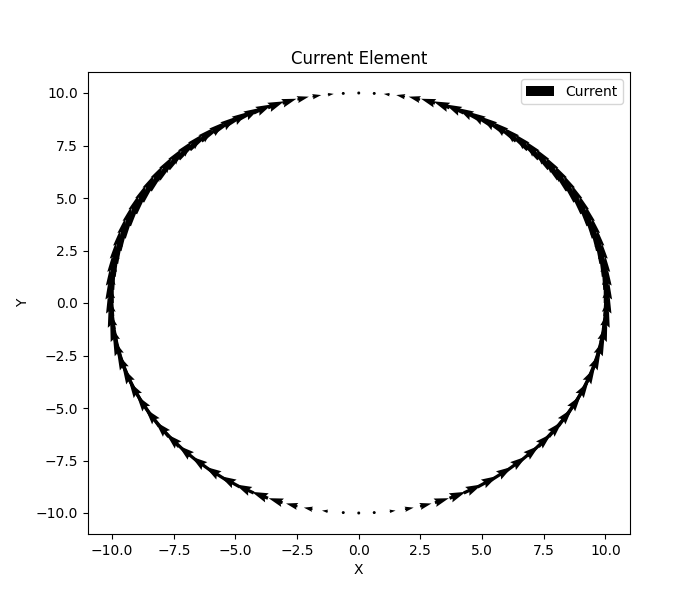
\includegraphics[scale=0.75]{Figure_1.png} 
	\label{fig:rawdata}
\end{center}
\clearpage

\section*{Vector Potential Calculation}
The vector potential of this system is given by
\begin{equation*}
\mathbf{A}_{ijk} = \sum_{l=0}^{N-1} \frac{cos(\phi_l)exp(-jkR_{ijk,l})\vec{dl_l}}{R_{ijk,l}}
\end{equation*}
where $R_{ijk,l}$ is the distance of each coordinate point $(X_i,Y_j,Z_k)$ from the $l^{th}$ current element. So 
\begin{equation*}
R_{ijk,l} = \sqrt{(X_i - x_l)^2 + (Y_j - y_l)^2 + (Z_k - z_l)^2}
\end{equation*}
Vectorially this can be reduced to
\begin{verbatim}
   R = ((X - r[0])**2 + (Y - r[1])**2 + (Z - r[2])**2)**(0.5)
\end{verbatim}
where the location of the $l^{th}$ current element is \texttt{r = r[0]}$\hat{x}$\texttt{ +  r[1]}$\hat{y}$\texttt{+ r[2]}$\hat{z}$. Thus the vector potential \texttt{Ax, Ay} can be calculated by
\begin{verbatim}
x = np.linspace(-1,1,Nx,dtype = float);
y = np.linspace(-1,1,Ny,dtype = float);
z = np.linspace(1,Nz,Nz,dtype = float);
Y,Z,X = np.meshgrid(y,z,x);

Ax = np.zeros((Nz,Ny,Nx))   
Ay = np.zeros((Nz,Ny,Nx))   

def calc(X,Y,Z, r, theta, IdL):
   R = ((X - r[0])**2 + (Y - r[1])**2 + (Z - r[2])**2)**(0.5)
   Ax = 1e-7*np.multiply(np.exp(-1j*R*k)/R, IdL[0])
   Ay = 1e-7*np.multiply(np.exp(-1j*R*k)/R, IdL[1])
   return Ax, Ay

for i in range(theta.size):
   AxTemp, AyTemp = calc(X,Y,Z, rL[:,i], theta[i], IdL[:,i])
   Ax = Ax + AxTemp
   Ay = Ay + AyTemp 

\end{verbatim}

\clearpage

\section*{Magnetic Field Calculation}

Once the vector potential is obtained the magnetic field is obtained from the equation $(6)$ as

\begin{verbatim}
delX = x[1] - x[0]
delY = y[1] - y[0]
Xmid = int(Nx/2)
Ymid = int(Ny/2)

B = (Ay[:,Ymid,Xmid+1] - Ay[:,Ymid,Xmid-1])/(2*delX) - 
    (Ax[:,Ymid+1,Xmid] - Ax[:,Ymid-1,Xmid])/(2*delY) 
B = np.abs(B)
\end{verbatim}

\begin{center}
	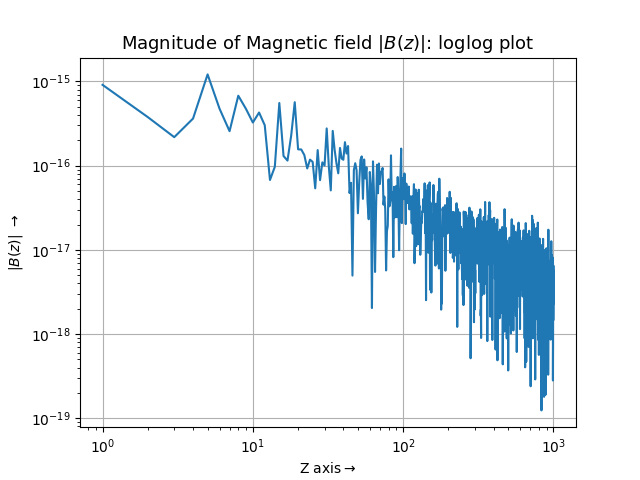
\includegraphics[scale=0.75]{Figure_2.png} 
	\label{fig:rawdata}
\end{center}

We can observe from the graph that the values for $B$ are very small in the orders of $10^{-16}$ which is approximately zero. The expected magnetic field is also \textbf{zero} since the current distribution $I_0cos(\phi)$ is symmetric about both $X$ and $Y$ axes. From the \textbf{Right Hand Rule} or \textbf{Cork Screw Rule}, the $B_z$ components cancel out and zero effect is observed. The small errors in the orders of $10^{-16}$ are due to the numerical errors/approximations during the calculations
\\

We try to fit the above mentioned graph into a loglog plot of the form:
\begin{align*}
B = Nz^{M} \\
\log B = \log N + M\log z
\end{align*}

\clearpage
 To estimate the values of $A$ and $b$ we use \textbf{least square method} such that the error in $B$ is minimum by using \texttt{scipy.linalg.lstsq} function. 

\begin{equation*}
\begin{pmatrix}
1 & z_1\\
1 & z_2\\
1 & z_3\\
.  .\\
.  .\\
1 & z_n\\
\end{pmatrix}
.
\begin{pmatrix}
\log(N)\\
M\\
\end{pmatrix}
=
\begin{pmatrix}
\log(B_1)\\
\log(B_2)\\
.\\
.\\
\log(B_n)\\
\end{pmatrix}
\end{equation*}

\begin{verbatim}
X = np.vstack([log(z), np.ones(len(z))]).T
M, N = scipy.linalg.lstsq(X, log(B))[0]
N = np.exp(N)
\end{verbatim}

By executing the code, we obtain the fit
\begin{verbatim}
When the graph is fitted in the form of B = Nz^M, we find:
N =  2.7786522586910982e-15
M =  -0.9731108586197116
\end{verbatim}

\begin{center}
	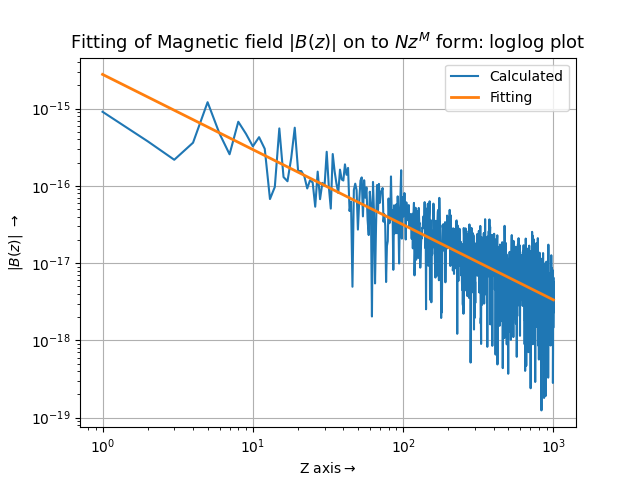
\includegraphics[scale=0.8]{Figure_3.png} 
	\label{fig:rawdata}
\end{center}

Since the expected $B_z$ is zero, no definite conclusion can be observed with just the numerical errors. 

In case of magnetostatics case, where the current doesn't vary with time - the expected $B_z$ field is \textbf{zero} as before since the system is symmetric. The static case is obtained by initializing \texttt{k = 0}
\clearpage

\begin{center}
	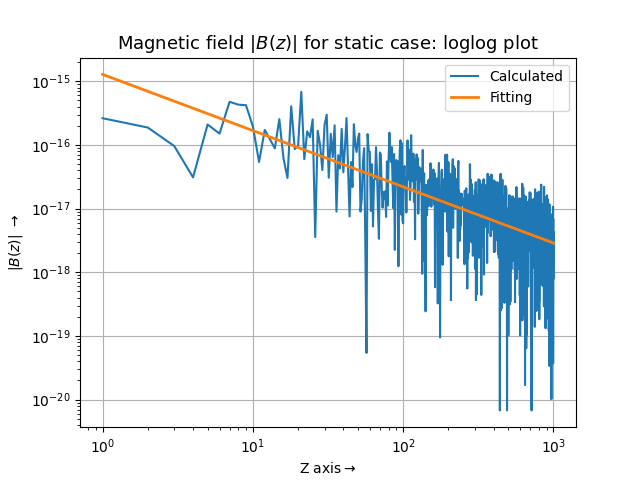
\includegraphics[scale=0.8]{Figure_4.png} 
	\label{fig:rawdata}
\end{center}

\begin{verbatim}
When the graph is fitted in the form of B = Nz^M, we find:
N =  1.2849960022740135e-15
M =  -0.8828302003695143
\end{verbatim}

As expected there is not much difference between $k = 0$ and $k \neq 0$ case.

\section*{Exploring Various Current Distributions}
In the previous pages, we have considered the current distribution to be both space and time variant with $I = I_0cos\phi exp(j\omega t)$. Now, Let us look into spatial, time invariant current distribution i.e., $I =$ $constant$. This condition can be observed by changing the code to
\begin{verbatim}
k = 0
I = np.ones(len(theta))*1e7
\end{verbatim}

The variation of magnetic field can be easily obtained by applying \textbf{Biot-Savart's Law}
\begin{equation*}
\mathbf{dB} = \frac{\mu_0 I \vec{dL} \times \hat{r}}{4\pi r^2}
\end{equation*}
where $\vec{r}$ is the vector from the current element to the position coordinate. On the z-axis, the $|\vec{r}|^2 = \sqrt{a^2 + z^2}$ where $a$ is the radius of the loop wire.
\clearpage

\begin{equation*}
dB_z = \frac{\mu_0 IdL}{4\pi}\frac{a}{(a^2 + z^2)^{3/2}}
\end{equation*}
\begin{equation*}
B_z = \frac{\mu_0 I_0}{2}\frac{a^2}{(a^2 + z^2)^{3/2}} \propto \frac{1}{z^3}
\end{equation*}

\begin{center}
	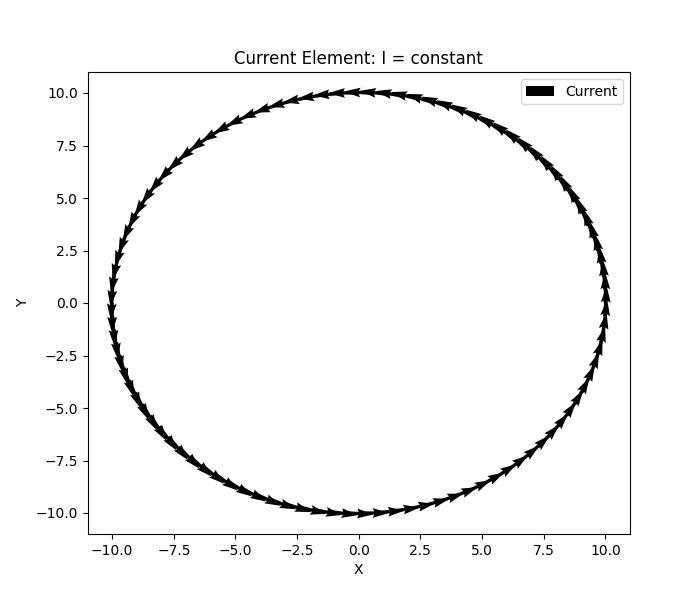
\includegraphics[scale=0.60]{Figure_15png.png} 
	\label{fig:rawdata}
\end{center}

\begin{center}
	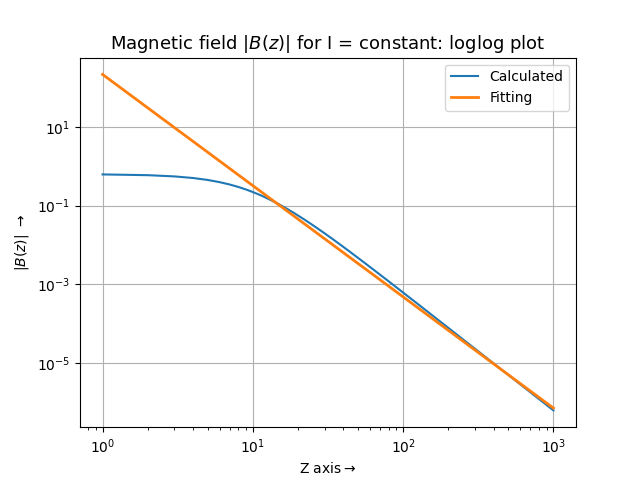
\includegraphics[scale=0.65]{Figure_5.png} 
	\label{fig:rawdata}
\end{center}

\begin{verbatim}
When the graph is fitted in the form of B = Nz^M, we find:
N =  215.85790244341976
M =  -2.826192056926644
\end{verbatim}
\clearpage
We observe from the graph that the magnetic value $B$ falls on the power of $z^{-2.82619}$ which is close to $z^{-3}$ as expected. Hence our simulation works well.
\\

Let us explore one another current distribution - time invariant but spatially varying
\begin{equation*}
I = \frac{4\pi}{\mu_0}|\cos({\phi})|
\end{equation*}
When the magnetic fields are plotted, we observe that
\begin{center}
	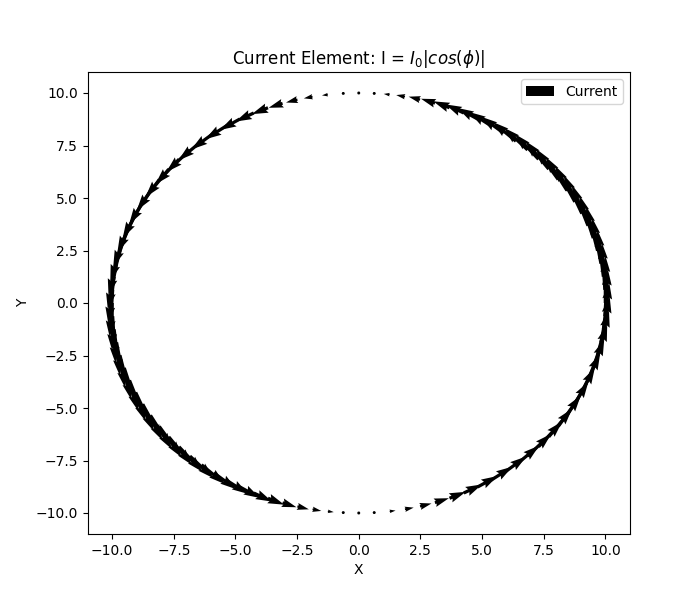
\includegraphics[scale=0.6]{Figure_6.png} 
	\label{fig:rawdata}
\end{center}
\begin{center}
	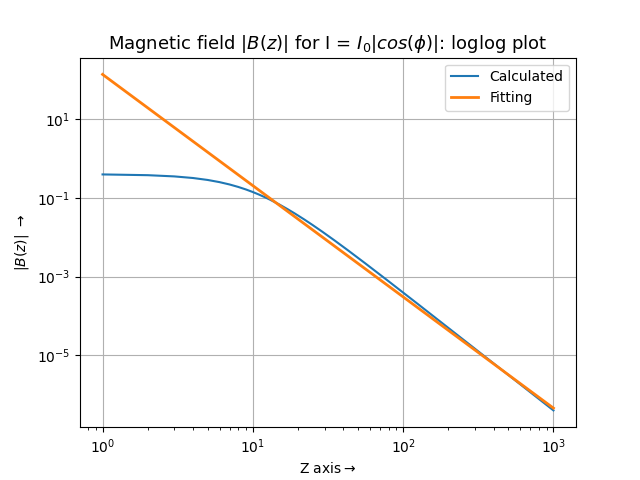
\includegraphics[scale=0.65]{Figure_7.png} 
	\label{fig:rawdata}
\end{center}

\begin{verbatim}
When the graph is fitted in the form of B = Nz^M, we find:
N =  137.36239855412188
M =  -2.8261780521825823
\end{verbatim}
We can observe that the $B$ falls on the power of $z^{-2.82619}$. Thus $B$ falls off as $\frac{1}{z^3}$

\section*{Conclusion}
For $I = I_0\cos({\phi})\exp({j\omega t})$ we plotted the current distribution, calculated the vector potential and magnetic potential. We observed that the values are in the order of $10^{-15}$. This is as expected since the expected magnetic field is zero. 
\\

We also tried to fit the magnetic field function in the form $B = Nz^M$ using \texttt{lstsq} function. Since the observed value are just numerical errors, no observable definite conclusions can be observed. We can observe the same for the magnetostatic time invariant case(k=0). 
\\

We also explored other current distributions like space time invariant distribution $I = I_0$. We observed that the magnetic field falls with $z^{-2.82}$ which is approximately the same as expected $z^{-3}$. We also plotted for the time invariant space variant distribution $I = I_0|\cos({\phi})|$ and observed that the field falls with $z^{-2.82}$. 
\\

Through this assignment, we learned on how to implement python arrays efficiently by vectorizing the loops. We also learnt how to implement Least Square Sum method using \texttt{lstsq} function
\clearpage

\end{document}

